\chapter{Stand van zaken}
\label{ch:stand-van-zaken}

% Tip: Begin elk hoofdstuk met een paragraaf inleiding die beschrijft hoe
% dit hoofdstuk past binnen het geheel van de bachelorproef. Geef in het
% bijzonder aan wat de link is met het vorige en volgende hoofdstuk.

% Pas na deze inleidende paragraaf komt de eerste sectiehoofding.

% Dit hoofdstuk bevat je literatuurstudie. De inhoud gaat verder op de inleiding, maar zal het onderwerp van de bachelorproef *diepgaand* uitspitten. De bedoeling is dat de lezer na lezing van dit hoofdstuk helemaal op de hoogte is van de huidige stand van zaken (state-of-the-art) in het onderzoeksdomein. Iemand die niet vertrouwd is met het onderwerp, weet er nu voldoende om de rest van het verhaal te kunnen volgen, zonder dat die er nog andere informatie moet over opzoeken \autocite{Pollefliet2011}.

% Je verwijst bij elke bewering die je doet, vakterm die je introduceert, enz. naar je bronnen. In \LaTeX{} kan dat met het commando \texttt{$\backslash${textcite\{\}}} of \texttt{$\backslash${autocite\{\}}}. Als argument van het commando geef je de ``sleutel'' van een ``record'' in een bibliografische databank in het Bib\TeX{}-formaat (een tekstbestand). Als je expliciet naar de auteur verwijst in de zin, gebruik je \texttt{$\backslash${}textcite\{\}}.
% Soms wil je de auteur niet expliciet vernoemen, dan gebruik je \texttt{$\backslash${}autocite\{\}}. In de volgende paragraaf een voorbeeld van elk.

% \textcite{Knuth1998} schreef een van de standaardwerken over sorteer- en zoekalgoritmen. Experten zijn het erover eens dat cloud computing een interessante opportuniteit vormen, zowel voor gebruikers als voor dienstverleners op vlak van informatietechnologie~\autocite{Creeger2009}.

Om een duidelijk inzicht te krijgen in wat de microservice architectuur is en wat zijn voordelen en pitfalls zijn, wordt in dit hoofdstuk een toelichting uiteengezet over deze architectuur. Daarna wordt beschreven welke technieken voor handen zijn om deze pitfalls van een antwoord te bieden. Meer bepaald technieken om te achterhalen hoe de flow van een bepaalde request door de applicatie propageert. 

Na het lezen van dit hoofdstuk moet je een goed begrip hebben over wat een microservice architectuur inhoudt en welke technologieën voor handen zijn om een antwoord te bieden op de problematiek rond tracing van requests. Deze kennis zal je nodig hebben om het verdere verloop van dit document vlot te kunnen volgen.

\section{MicroService architectuur}
Om een begrip te krijgen over wat de microservice architectuur inhoudt, dienen we eerst te weten wat een monolithische architectuur/applicatie is. Een monolithische architectuur ofwel een monolithische applicatie wordt gebouwd als een enkele eenheid. In bedrijfstoepassingen vindt men vaak drie hoofdonderdelen. Een client-side user interface, een databank en een server-side applicatie. De server-side applicatie is dan verantwoordelijk voor het afhandelen van \gls{HTTP-request}, het uitvoeren van domeinlogica, het ophalen en updaten van data in de databank en het genereren van HTML views om deze te verzenden naar de client. De server-side is hierbij een monolithische applicatie. In figuur \ref{fig:monolith} zie je een schematische voorstelling van een monolithische architectuur. Elke verandering aan het systeem vereist het opnieuw builden en deployen van de server-side applicatie.

\begin{figure}
	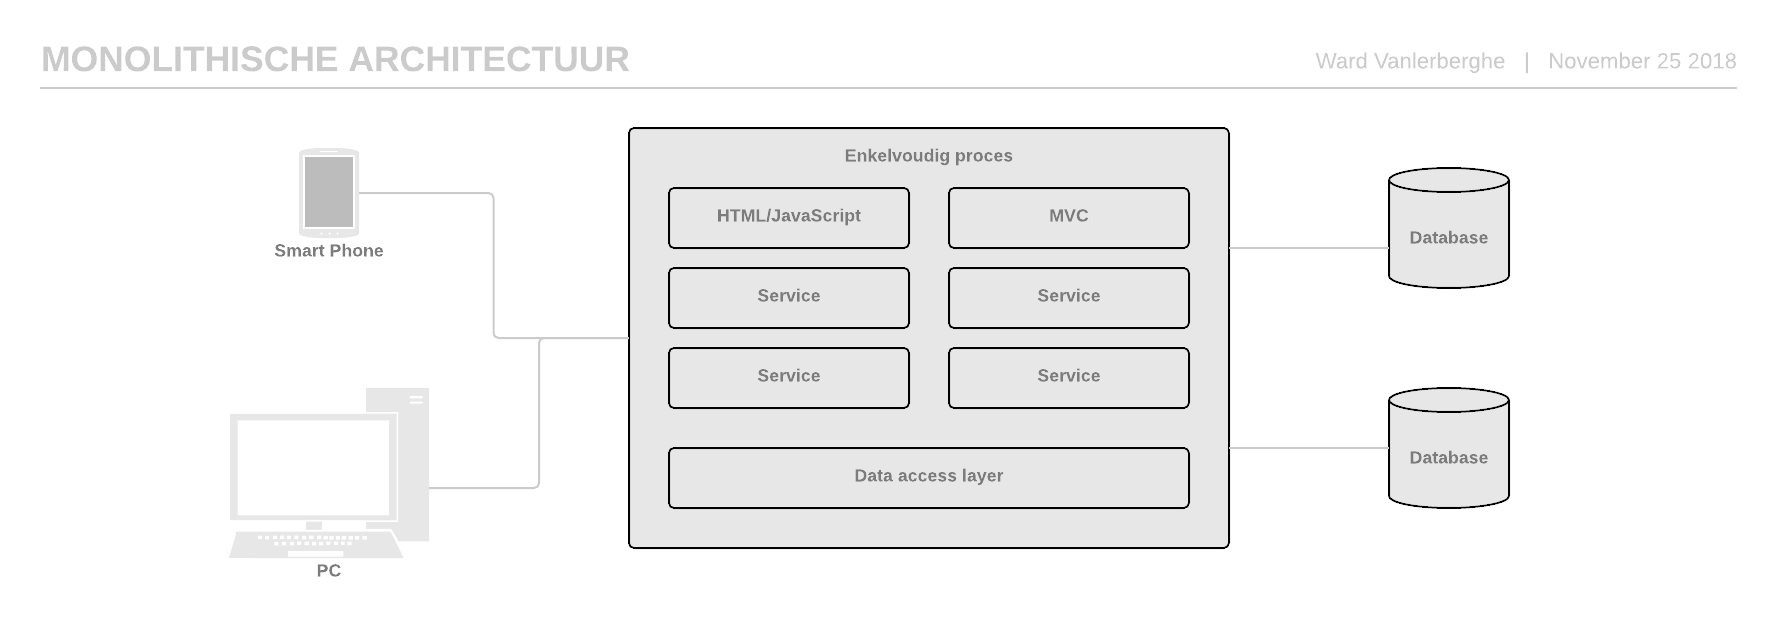
\includegraphics[width=\linewidth]{img/monolith.png}
	\caption{Weergave van een applicatie die gebruik maakt van een monolithische architectuur}
	\label{fig:monolith}
\end{figure}

Al de logica om een request af te handelen runt in één proces. Monolithische applicaties kunnen succesvol zijn. Echter meer en meer mensen voelen frustratie bij dergelijke applicaties, vooral met de toename van het deployen van applicaties naar de cloud. Elke verandering aan een kleine module van de applicatie vereist het opnieuw builden en deployen van de volledige monolithische applicatie. Na verloop van tijd word het moeilijk om een goede modulaire structuur te behouden en veranderingen die slechts aan een enkele module dienen te gebeuren worden steeds moeilijker. Indien een bepaalde module meer resources vereist dient de volledige monoliet geschaald te worden in plaats van enkel die bepaalde module. \autocite{Fowler2014}

Door deze frustraties zijn developers beginnen zoeken naar alternatieve manieren om applicaties te ontwikkelen. Dit heeft geleidt tot de microservice architectuur. Bij een microservice architectuur worden applicaties gebouwd als een verzameling van services die onafhankelijk van elkaar kunnen worden gedeployed en gescaled. Deze services communiceren doorgaans met elkaar via een \gls{REST API}. Elke service heeft een grondig afgebakende scope en volgens \textcite{Fowler2014} een eigen databank. Hoewel dit laatste niet echt een vereiste is. Echter vergt het veel discipline van de developer indien er met een gedeelde databank wordt gewerkt \autocite{Young2016}. In figuur \ref{fig:microservices} vind je een schematische voorstelling terug van een microservice architectuur.

\begin{figure}
	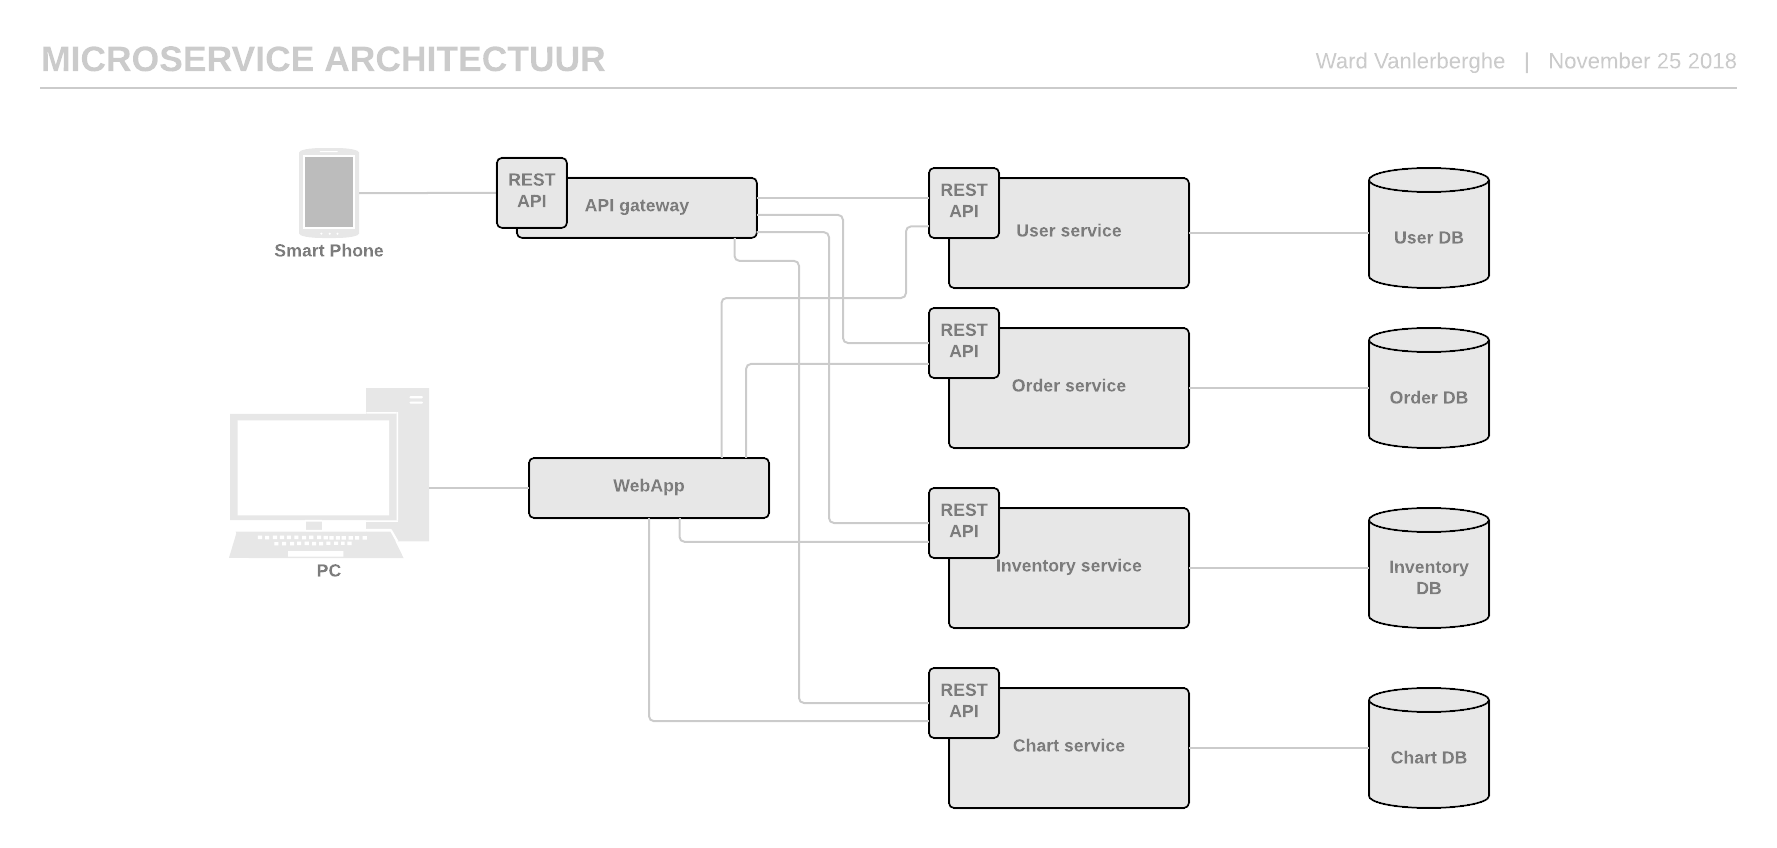
\includegraphics[width=\linewidth]{img/microservices.png}
	\caption{Weergave van een applicatie die gebruik maakt van een microservice architectuur}
	\label{fig:microservices}
\end{figure}

\section{De voordelen van een MicroService architectuur}
Zoals reeds eerder in dit hoofdstuk vermeld heeft een microservice architectuur tal van voordelen ten opzichte van een monolithische architectuur. En deze voordelen worden enkel maar groter naar gelang een applicatie groeit. Doordat de services op zo een manier van elkaar ontkoppelt zijn, is het mogelijk om voor elke service een andere programmeertaal of databanktechnologie te gebruiken. Door de modulariteit van deze architectuur kan een zeer hoge availability gegarandeerd worden, het falen van een bepaalde service hoeft niet te betekenen dat de rest van de applicatie niet bruikbaar is. Enkel de module die faalt zal tijdelijk niet toegankelijk zijn voor de eindgebruiker van de applicatie. Tevens is het veel eenvoudiger om functionaliteit aan een applicatie toe te voegen zonder de werking van de andere services (op een negatieve manier) te beïnvloeden.

Omdat de services in verschillende processen draaien wordt het ook een stuk makkelijker om DevOps methodologieën te gaan gebruiken en de \gls{CI} en \gls{CD} principes gaan toe te passen. Deployen van nieuwe of gewijzigde functionaliteit hoeft hier geen downtime van de applicatie te betekenen.

Zoals je merkt zijn de voordelen van een microservice architectuur groot. Er zijn natuurlijk nog veel meer voordelen dan dat hier staat beschreven, maar hier nog dieper op ingaan valt buiten de scope van dit onderzoek.

In alle eerlijkheid is de microservice architectuur lang geen nieuw concept, zo  wordt beweert dat microservices hetzelfde is als \gls{SOA}, maar dan op een correcte manier uitgevoerd \autocite{Morris2014} \autocite{Young2016}. In een talk op microCon zegt \textcite{Young2016} zelfs dat het concept van microservices dateert van reeds 5 decennia geleden.

\section{De pitfalls van een MicroService architectuur}
Zoals bij vele methodieken in softwareontwikkeling, heeft ook de microservice architectuur zijn nadelen. Het is makkelijk in te beelden dat een applicatie met een groot aantal microservices al gauw zeer complex wordt.

De grote nadelen volgens \textcite{Fowler2015} en \textcite{Hummel2018} zijn:

\begin{itemize}
	\item Verschillende databanken en transactie management kunnen een pijnpunt vormen.
	\item Het testen van een applicatie met een microservice architectuur kan zeer moeizaam zijn. Dit komt omdat we voor elke microservice moeten confirmeren of deze daadwerkelijk in een healthy state is vooraleer we kunnen van start gaan met testen.
	\item Het deployen van microservices kan complex zijn. Ze kunnen coördinatie nodig hebben tussen verschillende services en extra configuratie vereisen.
	\item Het ontwikkelen van \gls{gedistribueerde systemen} kan complex zijn. Aangezien alles nu een onafhankelijke service is, moet je er voor zorgen dat elke request op een correcte manier doorheen de verschillende services propageert. Na verloop van tijd zullen complicaties ontstaan waarbij \gls{HTTP-request} onderhevig zijn aan hoge latencies.
\end{itemize}

Voor elk van deze nadelen bestaat er natuurlijk een oplossing \autocite{Hummel2018}. In dit onderzoek gaan we met name twee tools bespreken en vergelijken om op de laatste pitfall uit bovenstaande lijst een antwoord te bieden.

\section{Distributed Tracing}
Distributed tracing is een methode om applicaties te monitoren, hoofdzakelijk applicaties die gebruik maken van de microservice architectuur. Door het instrumenteren van code ontstaat een zogenaamde \gls{trace}. Deze \gls{trace} geeft ons informatie over de performantie van het systeem in de vorm van \gls{span}s. Bv. hoe lang een bepaalde request nodig heeft om antwoord te geven aan de caller. Een \gls{span} is hierbij de metadata van een unit of work voor een bepaalde \gls{REST} call, uitvoering van een methode, databank call,...

Op deze manier kunnen we dus belangrijke informatie vergaren over de werking van het systeem. Door het analyseren van deze \gls{trace}s kunnen we de code van de applicatie optimaliseren en latencies van requests verlagen.

Distributed tracing is geen nieuw concept, Google bracht in 2010 reeds de paper \begin{quotation}
	"Dapper, a Large-Scale Distributed Systems Tracing Infrastructure"
\end{quotation} uit \autocite{36356}. Waarin de auteurs de nood van distributed tracing beschrijven en hoe ze dit hebben aangepakt binnen Google. Deze paper ligt aan de basis van veel distributed tracing tools vandaag voor handen \autocite{Mace2017}.

\section{OpenTracing}
Het grote probleem dat ontstond bij distributed tracing was dat elke tool zijn eigen implementatie van een \gls{trace} had. Hierdoor was het niet makkelijk om in een lopend project van tooling te veranderen indien de tool niet langer aan de verwachtingen van het systeem voldeed. Er ontstond als het ware een vendor lock-in.

De nood om een standaard te ontwikkelen die het mogelijk maakt om een applicatie te instrumenteren zonder vast te hangen aan een bepaalde tool was dus groot. In deze optiek werd OpenTracing\footnote{https://opentracing.io/} ontwikkeld onder de vlag van \gls{CNCF}\footnote{https://www.cncf.io/}. OpenTracing is een standaard die developers van applicaties, \gls{OSS} packages en \gls{OSS} services, toelaat om hun code te instrumenteren zonder zich aan een bepaalde tracing vendor te binden. Eerdere pogingen om een standaard te creëren voor distributed tracing focusten zich enkel op het encoderen en representatie van de \gls{trace} en context data. Zowel inkomende als uitgaande. Echter is dit niet voldoende om een vendor lock-in te vermijden \autocite{Sigelman2016}.

OpenTracing biedt met name volgende standaarden aan om dit toch te verwezenlijken \autocite{Sigelman2016}:

\begin{itemize}
	\item \textbf{Gestandaardiseerde \gls{span} management:} programmatische \gls{API}'s om getimede operaties te starten, te stoppen en te decoreren ("\gls{span}s")
	\item \textbf{Gestandaardiseerde inter-proces propagatie:} programmatische \gls{API}'s om hulp te bieden bij het doorgeven van de tracing context over de grenzen van een proces heen
	\item \textbf{Gestandaardiseerde active \gls{span} management:} programmatische \gls{API}'s om de actieve \gls{span} op te slaan en op te vragen over de grenzen van packages die in een single process draaien
	\item \textbf{Gestandaardiseerde in-band context encodering:} specificatie van het encoderingsformaat van de tracing context die tussen processen wordt doorgegeven
	\item \textbf{Gestandaardiseerde out-of-band \gls{trace} data encodering:} specificatie van de gedecoreerde \gls{trace} en \gls{span} data encodering die naar de distributed tracing tool gepropageerd wordt
\end{itemize}

Sinds de opkomst van OpenTracing zijn er veel tools die deze standaard zijn beginnen te ondersteunen. Alsook Zipkin en Jeager, de twee tools die in de volgende hoofdstukken verder zullen worden uitgediept.